
\section{Training the models} % ----------------------------------------------
The training phase is divided in two parts, where two different optimizers were used: 
\begin{itemize}
    \item ResNet tail training using SGD, which is the only architecture that requires to be trained from scratch, whereas EfficientNet and MobileNet use pre-trained weighs.
    \item Training the heads of the other configurations with Adam, with both the baseline HP heads and the optimized ones. 
\end{itemize}


\noindent
In both phases, the MSE loss function is used, which, despite being more sensitive to outliers, converges quicker than the MAE loss. Moreover, both loss functions were tested and MSE consistently yielded better-performing models in a smaller number of epochs.\\

\noindent
In order to train our custom ResNet from scratch, the SGD optimizer is used with mostly the same HPs as in \cite{resnet2016}, minus the learning rate, which is two orders of magnitude smaller due to the fact that our network is shallower than the original one. 
Additionally, there are no head layers attached during this phase, thus the two output units are connected directly to the flattened output of the CNN.
The SGD HPs used for training are:
\begin{itemize}
    \item \textbf{Learning rate:} $\eta =1\times 10^{-3}$, with a plateau decaying factor of 0.2, meaning that if during training the validation loss becomes stationary, the LR is reduced to allow for finer gradient steps necessary for converging to a local minima.
    \item \textbf{Momentum:} $\beta = 0.9$, which applies gradient smoothing using a weighted moving average on the succession of gradients. Formally:
    \begin{equation*}
    \centering
        \begin{gathered}
        m_t = \beta m_{t-1} + \eta_t\nabla L(W_t)  \\
        W_{t+1} = W_t - m_t\\
        \end{gathered}
    \end{equation*}
    Where $m_t$ is the gradient computed at time $t$, $W_t$ are the weights of the network, $\nabla L$ is the loss gradient (computed wrt. a random extraction of one datapoint), $\eta_t$ is the learning rate, and $\beta$ is the momentum.
    \item \textbf{Weight Decay:} $\lambda =1\times10^{-4}$, is a regularization technique which consists in adding to the loss a penalty term proportional to the L2 norm of the weights in the network.\\
    Putting it all together, the penalty term and final weight update become:
    \begin{equation*}
    \centering
        \begin{gathered}
        L_{\lambda}(W_t) = L(W_t) + \frac{\lambda}{2}||W_t||^2  \\
        W_{t+1} = W_t - m_t - \eta_t\lambda W_t\\
        \end{gathered}
    \end{equation*}
     
\end{itemize}

\noindent
During the head training phase, the Adam optimizer is used, which combines the momentum technique described above with \textit{RMSProp}, which is a similar technique but considers the weighted moving average of the squared gradients:
    $$
        V_t = \gamma V_{t-1} + \eta_t(\nabla L(W_t))^2  
    $$
Where $\gamma$ is the discounting factor, similar to the $\beta$ factor of momentum. Then, the squared root of this moving average is used to adaptively reduce the learning rate, and the update rule for the weights becomes:
    $$
        W_{t+1} = W_t - \frac{m_t}{\sqrt{V_t + \varepsilon}}
    $$
This ensures that each weight of the network is adjusted adaptively, with momentum smoothing and scaled updates in case of large gradients\footnote{The additional bias correction steps for the $m_t$ and $V_t$ terms were omitted for brevity.}. The stopping criterion for each run is EarlyStopping, with a patience of 7 epochs, and, after stopping the training process, the best weights (i.e., those that minimize validation loss) are restored and saved to disk.

\subsection{Training results} % ----------------------------------------------

\noindent
The HyperBand parameters chosen for the HP optimization phase, allow us to test 17 different HP configurations, with a maximum trial amount of 50. The time needed to optimize each head depends heavily on the total number of parameters of the model, thus optimizing ResNet requires approximately 30 minutes, whereas optimizing EfficientNet requires up to five hours.


The number of parameters and the inference time of the optimized models are summarized in \textbf{Table \ref{tab:inference_times}}, where the GPU used for these tests is an RTX2080 and the CPU an i7-9700K. The times reported are relative to a single datapoint; calculated by dividing the inference time of a batch by its cardinality.
\begin{table}[ht!]
    \centering
    \newcolumntype{Y}{>{\centering\arraybackslash}X}
    \begin{tabularx}{\textwidth}{YYYYY}
        \hline
        \textbf{Model}              & \textbf{Tail params}  & \textbf{Head params} & \textbf{t-GPU(ms)} & \textbf{t-CPU(ms)}\\
            \hline 
            \textbf{ResNet}         & \num{389760}          & \num{135170}      & 0.6  & 4.2 \\ 
            \textbf{EfficientNet}   & \num{12930622}        & \num{1511170}     & 15.2 & 562  \\ 
            \textbf{MobileNet}      & \num{2996352}         & \num{542274}      & 4.5  & 250  \\ \hline
    \end{tabularx}
    \captionof{table}{Parameters count and inference time of each optimized model.}
    \label{tab:inference_times}
\end{table}


\noindent
After having optimized each model, a training run is performed with the best HPs and $k$-fold cross validation is used to obtain robust estimates for the model performances. The results are summarized in \textbf{Table \ref{tab:perf_comparison}}, where we can observe how the ResNet optimized model outperforms the others, with respect to both the test and cross validation losses. While EfficientNet follows closely the performance of ResNet, MobileNet performs well on the test set but has a really high cross validation loss, which indicates that it may have a tendency to overfit on the training data, preventing it from generalize as well as the other models.


\begin{table}[ht!]
    \centering
    \newcolumntype{Y}{>{\centering\arraybackslash}X}
    \begin{tabularx}{\textwidth}{YYYYY}
        \hline
        \textbf{Model}       & \textbf{Train Loss} & \textbf{Val Loss} & \textbf{Test Loss} & \textbf{5-fold CV}\\
            \hline 
            \textbf{ResNet}             &  &  &  & \\
            Baseline        & 0.0368      & 0.0365              & 0.0354            & 0.0416\\ 
            Optimized       & 0.0366      & \bt{0.0358}         & \bt{0.0352}       & \bt{0.0367}\\ 
                \hline
             
            \textbf{EfficientNet}       &  &  & & \\
            Baseline        & 0.0355      & 0.0370              & 0.0364            & 0.0382 \\ 
            Optimized       & 0.0351      & 0.0361              & 0.0363            & 0.0376 \\ 
                \hline
             
            \textbf{MobileNet}          &  &  & & \\
            Baseline        & 0.0261      & 0.0417              & 0.0452            & 0.0471 \\ 
            Optimized       & 0.0359      & 0.0362              & 0.0356            & 0.0519 \\ 
                \hline
    \end{tabularx}
    \captionof{table}{Baseline vs optimized performance of the three CNNs.}
    \label{tab:perf_comparison}
\end{table}
\noindent
In summary, a shallow ResNet trained from scratch on a small dataset outperforms more complex pre-trained architectures. This indicates that our learning task is sufficiently easy, likely due to the visual simplicity of the images, combined with a good correlation between the structural characteristics of an environment and the resulting ATE/ARE values.\\

\noindent
\textbf{Figure \ref{fig:train_perf}} shows the training and validation loss curves observed for both baseline and optimized heads, where we can observe how the optimized architectures converge very quickly to a lower validation loss than their baseline counterparts. In fact, the baseline architectures require at least 10 to 15 epochs for the validation losses to become stationary, whereas the optimized ones require around 5 epochs. As an example of a poor training result, \textbf{Figure \ref{fig:train_perf}e} shows how the MobileNet head with baseline parameters overfits, which is deducible by the validation loss increase after the 20 epoch mark, while the training loss keeps decreasing. 

\noindent
Moreover, as shown in \textbf{Figure \ref{fig:train_perf}e} and \textbf{Figure \ref{fig:train_perf}c}, the validation losses are fairly noisy before convergence, whereas their optimized counterparts appear to converge in a smoother fashion.  


\begin{figure}[ht!]
    \centering
        \subfloat[Baseline ResNet]{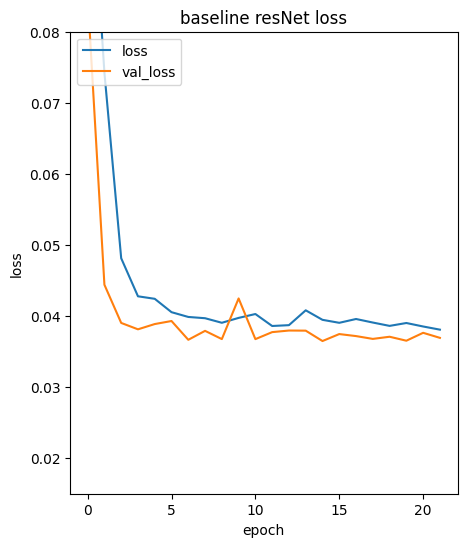
\includegraphics[height=.45\linewidth]{images/res_base.png}}\hspace{1cm}
        \subfloat[Optimized ResNet]{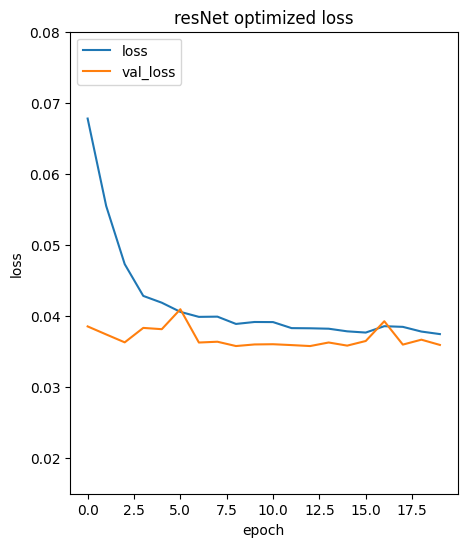
\includegraphics[height=.45\linewidth]{images/res_opt.png}}\hfill
        \subfloat[Baseline EfficientNet]{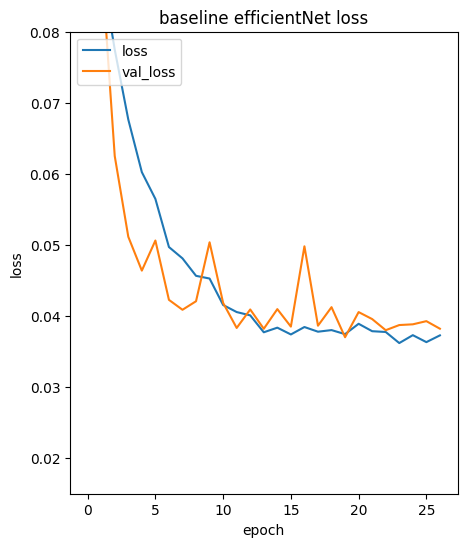
\includegraphics[height=.45\linewidth]{images/eff_base.png}}\hspace{1cm}
        \subfloat[Optimized EfficientNet]{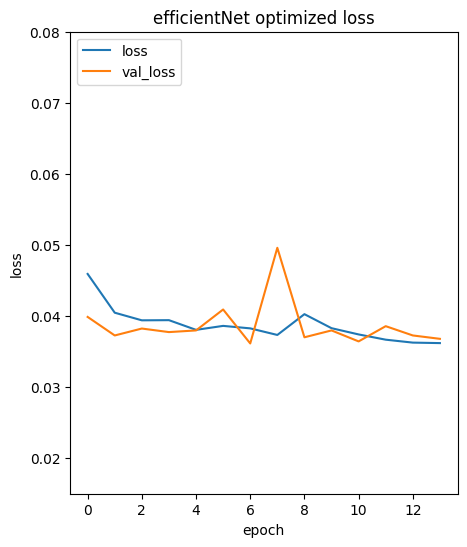
\includegraphics[height=.45\linewidth]{images/eff_opt.png}}\hfill
        \subfloat[Baseline MobileNet]{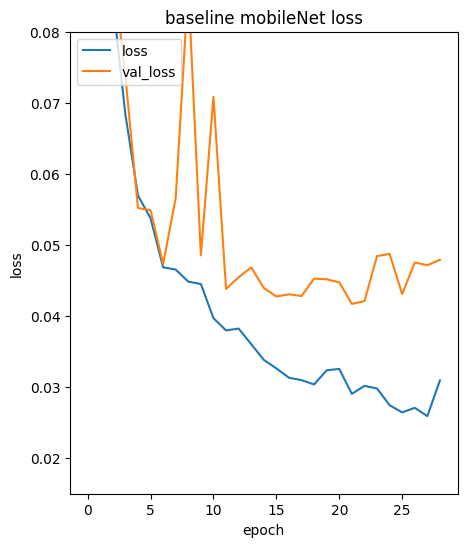
\includegraphics[height=.45\linewidth]{images/mob_base.png}}\hspace{1cm}
        \subfloat[Optimized MobileNet]{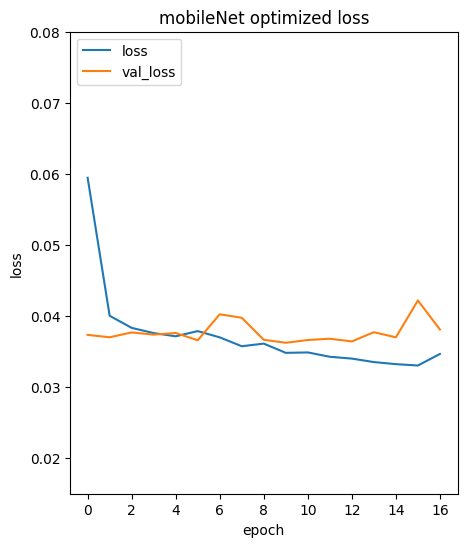
\includegraphics[height=.45\linewidth]{images/mob_opt.png}}
    \caption{Training curves of the various models}\label{fig:train_perf}
\end{figure}

\newpage